\begin{previewactivity}[\textbf{Functions with Finite Domains}] \label{PA:functionswithfinitedom} \hfill \\
Let  $A$  and  $B$  be sets.  Given a function  $f\x A \to B$, we know the following:

\begin{itemize}
\item For every  $x \in A$, $f( x ) \in B$.  That is, every element of  $A$  is an input for the function  $f$.  This could also be stated as follows:  For each  $x \in A$, there exists a  $y \in B$ such that  $y = f( x )$.

\item For a given $x  \in A$, there is exactly one  $y \in B$ such that  $y = f( x )$.

\end{itemize}
%\pagebreak
The definition of a function does not require that different inputs produce different outputs.  That is, it is possible to have  $x_1 , x_2  \in A$ with  
$x_1  \ne x_2 $ and  $f( {x_1 } ) = f( {x_2 } )$.  The arrow diagram for the function $f$ in Figure~\ref{fig:arrow63-1new} illustrates such a function.

\begin{figure}[h]
\begin{center}
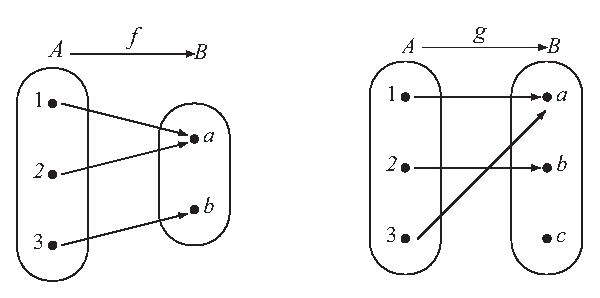
\includegraphics{figps-arrow63-1new.eps} 
\caption{Arrow Diagram for Two Functions} \label{fig:arrow63-1new}
\end{center}
\end{figure}

Also, the definition of a function does not require that the range of the function must equal the codomain.  The range is always a subset of the codomain, but these two sets are not required to be equal.  That is, if  
$g\x A \to B$, then it is possible to have a  $y \in B$ such that  $g( x ) \ne y$ for all  $x \in A$.  The arrow diagram for the function $g$ in Figure~\ref{fig:arrow63-1new} illustrates such a function.

Now let  $A = \left\{ {1,2,3} \right\}$, $B = \left\{ {a,b,c,d} \right\}$, and 
$C = \left\{ {s,t} \right\}$.  Define

\begin{center}
\begin{tabular}{c | c | c}
$f\x A \to B$ by &  $g\x A \to B$ by &  $h\x A \to C$ by \\
$f( 1 ) = a $  &  $g( 1 ) = a $  &  $h( 1 ) = s $ \\
$f( 2 ) = b $  &  $g( 2 ) = b $  &  $h( 2 ) = t $ \\
$f( 3 ) = c $  &  $g( 3 ) = a $  &  $h( 3 ) = s $
\end{tabular}
\end{center}
%
\begin{enumerate}
\item Which of these functions satisfy the following property for a function  $F$?

\begin{list}{}
\item For all  $x, y \in \text{dom}( F )$, if  $x \ne y$, then  
$F(x) \ne F(y)$.
\end{list}

\item Which of these functions satisfy the following property for a function  $F$?

\begin{list}{}
\item For all  $x, y \in \text{dom}( F )$, if  
$F( x ) = F( y )$, then  $x = y$.
\end{list}

\item Determine the range of each of these functions.

\item Which of these functions have their range equal to their codomain?

\item Which of the these functions satisfy the following property for a function  $F$?

\begin{list}{}
\item For all  $y$ in the codomain of $F$, there exists an  
$x \in \text{dom}( F )$ such that  $F( x ) = y$.
\end{list}
\end{enumerate}
\end{previewactivity}
\hbreak

\endinput
